\documentclass{beamer}
%% \documentclass[draft]{beamer} %% draft version

%% restrict generation of slides
%% \includeonlyframes{oligoarray,probesyn}

\mode<presentation>
{
  \usetheme{Bielefeld}
  \setbeamercovered{transparent}
}

\usepackage[english]{babel}
\usepackage[latin1]{inputenc}
\usepackage{graphicx}

\usepackage{lmodern}
\usepackage[T1]{fontenc}

\newcommand{\ignore}[1]{}

\title[GCB 2006 - Microarray Layout as a Quadratic Assignment Problem] % (optional, use only with long paper titles)
{Microarray Layout as a Quadratic Assignment Problem}

%% \subtitle
%% {Include Only If Paper Has a Subtitle}

\author[S.~A.~de~Carvalho~Jr. (Universit\"at Bielefeld)] % (optional, use only with lots of authors)
{S\'ergio A. de Carvalho Jr.\inst{1,}\inst{2}\inst{,3} \and Sven Rahmann\inst{1,}\inst{2}}
% - Give the names in the same order as the appear in the paper.
% - Use the \inst{?} command only if the authors have different
%   affiliation.

\institute[Universit\"{a}t Bielefeld] % (optional, but mostly needed)
{
\inst{1}%
Algorithms and Statistics for Systems Biology, Genome Informatics,\\
Technische Fakult\"at, Universit\"at Bielefeld, Germany
\and
\inst{2}%
International NRW Graduate School in Bioinformatics and Genome Research
\and
\inst{3}%
Graduiertenkolleg Bioinformatik
}
% - Use the \inst command only if there are several affiliations.
% - Keep it simple, no one is interested in your street address.

\date[GCB 2006] % (optional, should be abbreviation of conference name)
{German Conference on Bioinformatics, 2006}
% - Either use conference name or its abbreviation.
% - Not really informative to the audience, more for people (including
%   yourself) who are reading the slides online

% \subject{Theoretical Computer Science}
% This is only inserted into the PDF information catalog. Can be left
% out. 

% If you have a file called "university-logo-filename.xxx", where xxx
% is a graphic format that can be processed by latex or pdflatex,
% resp., then you can add a logo as follows:

% \pgfdeclareimage[height=0.5cm]{university-logo}{university-logo-filename}
% \logo{\pgfuseimage{university-logo}}

% Delete this, if you do not want the table of contents to pop up at
% the beginning of each subsection:
\AtBeginSubsection[]
{
  \begin{frame}<beamer>
    \frametitle{Outline}
    \tableofcontents[currentsection,hideallsubsections]
  \end{frame}
}

% If you wish to uncover everything in a step-wise fashion, uncomment
% the following command: 
%\beamerdefaultoverlayspecification{<+->}


\begin{document}

%%%%%%%%%%%%%%%%%%%%%%%%%%%%%%%%%%%%%%%%%%%%%%%%%%%%%%%%%%%%%%%%%%%%%%%%%%%%%%%%
\frame[plain]{

  \vspace*{0.4cm}
  \centerline{
    
\includegraphics[height=1.3cm]{pics/aggi_logo.png}
    \hspace*{0.6cm}
    
\includegraphics[height=1.3cm]{pics/gsbg_logo.png}
  }
  
  \titlepage
}

%%%%%%%%%%%%%%%%%%%%%%%%%%%%%%%%%%%%%%%%%%%%%%%%%%%%%%%%%%%%%%%%%%%%%%%%%%%%%%%%
\frame{\frametitle{Outline}

  \tableofcontents[hideallsubsections]

}

%% *****************************************************************************
\section[Introduction]{Introduction to Microarray Layout}
\subsection{Dummy}
%% *****************************************************************************

%%%%%%%%%%%%%%%%%%%%%%%%%%%%%%%%%%%%%%%%%%%%%%%%%%%%%%%%%%%%%%%%%%%%%%%%%%%%%%%%
\frame[label=oligoarray]{\frametitle{High-Density Oligonucleotide Microarrays}

  \centerline{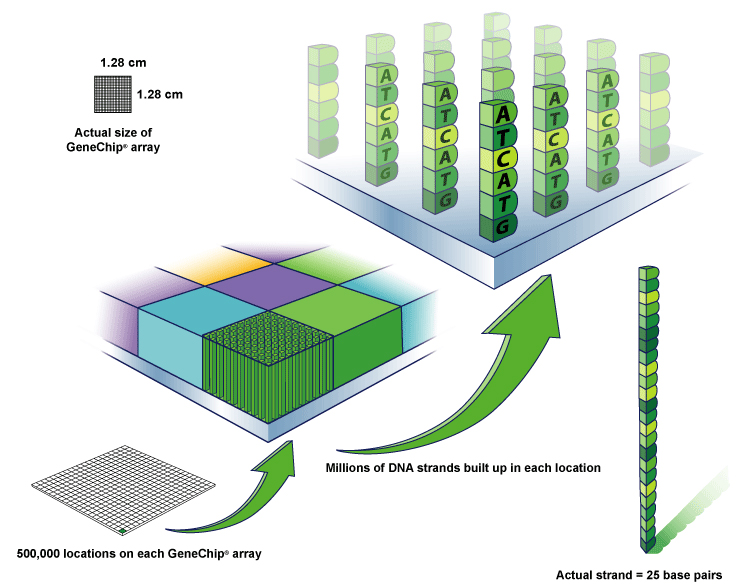
\includegraphics[height=0.9\textheight]{pics/oligoarray.jpg}}
  \vspace*{-0.5cm}
  \centerline{\tiny{Source: Affymetrix, Inc.}}

}

%%%%%%%%%%%%%%%%%%%%%%%%%%%%%%%%%%%%%%%%%%%%%%%%%%%%%%%%%%%%%%%%%%%%%%%%%%%%%%%%
\frame[label=probesyn]{\frametitle{Probe Synthesis with Photolitographic Masks}

  \vspace*{-0.5cm}
  \flushright{\tiny{Source: Affymetrix, Inc.}}
  \centerline{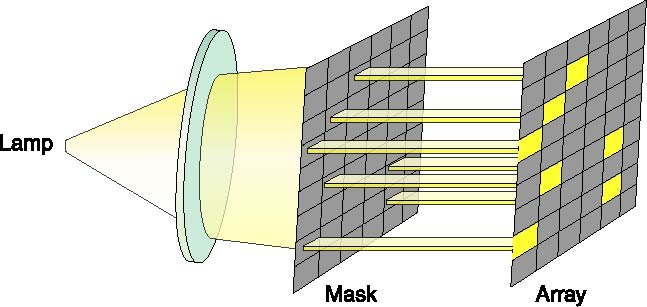
\includegraphics[height=0.5\textheight]{pics/photolithography.jpg}}  

  \begin{itemize}
    \item Probes are synthesized on the chip in a \alert{series of steps}
    \item Each step \alert{appends a particular nucleotide} to selected regions
    \item Selection occurs by exposure to light directed by a \alert{mask}
  \end{itemize}
}

%%%%%%%%%%%%%%%%%%%%%%%%%%%%%%%%%%%%%%%%%%%%%%%%%%%%%%%%%%%%%%%%%%%%%%%%%%%%%%%%
\frame[label=embed]{\frametitle{Deposition Sequence and Probe Embeddings}

  \begin{overprint}
  \onslide<+>
    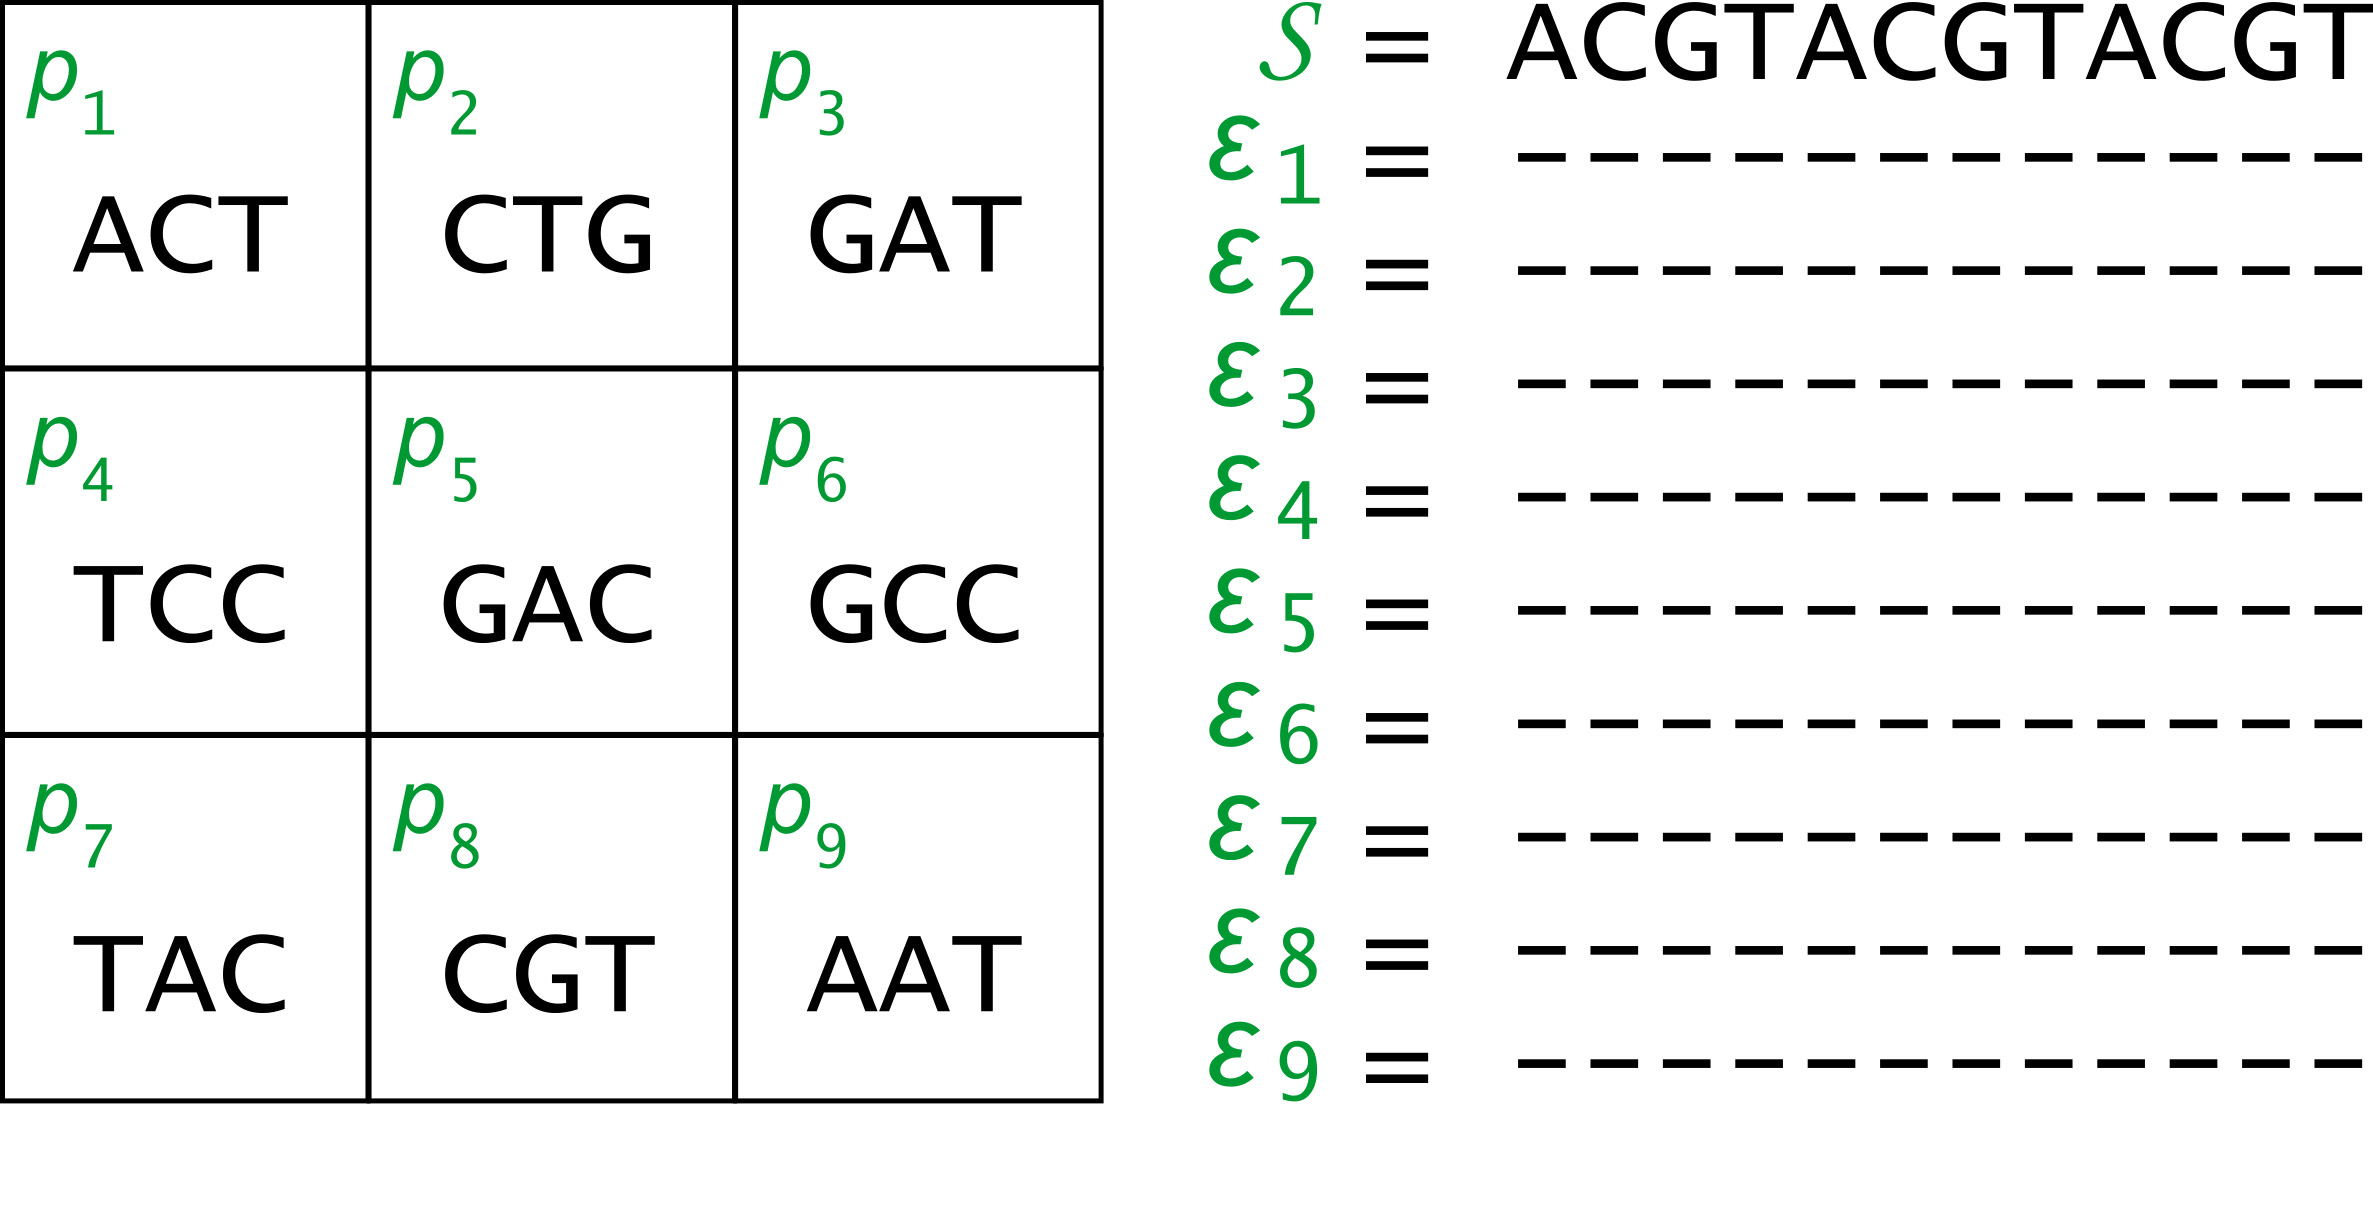
\includegraphics[width=\textwidth]{masks/chip.jpg}
  \onslide<+>
    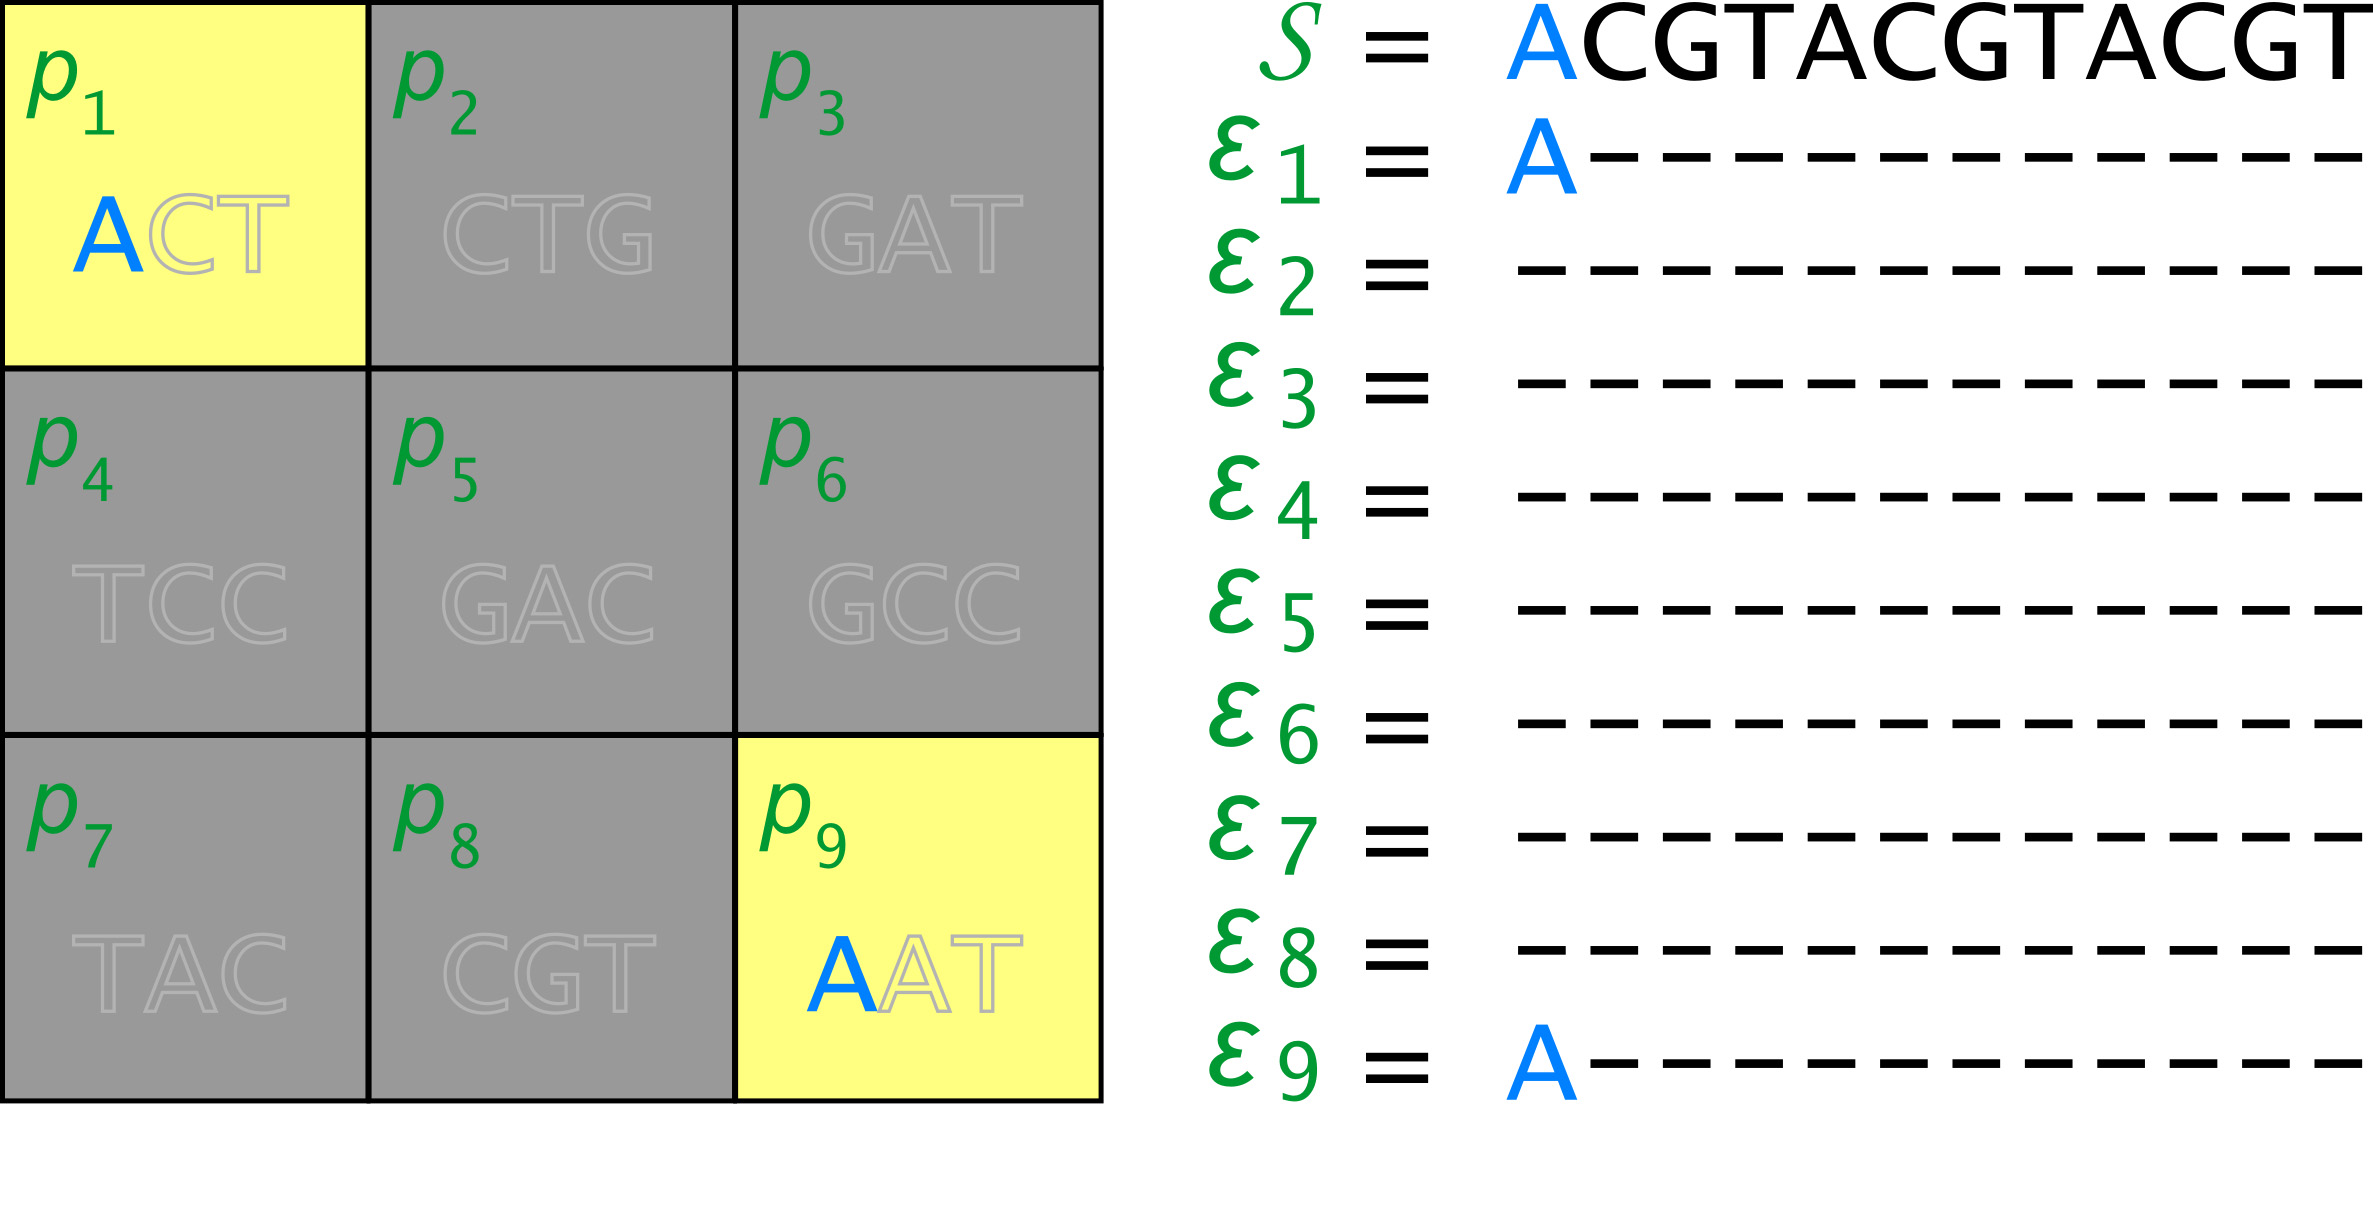
\includegraphics[width=\textwidth]{masks/mask1.jpg}
  \onslide<+>
    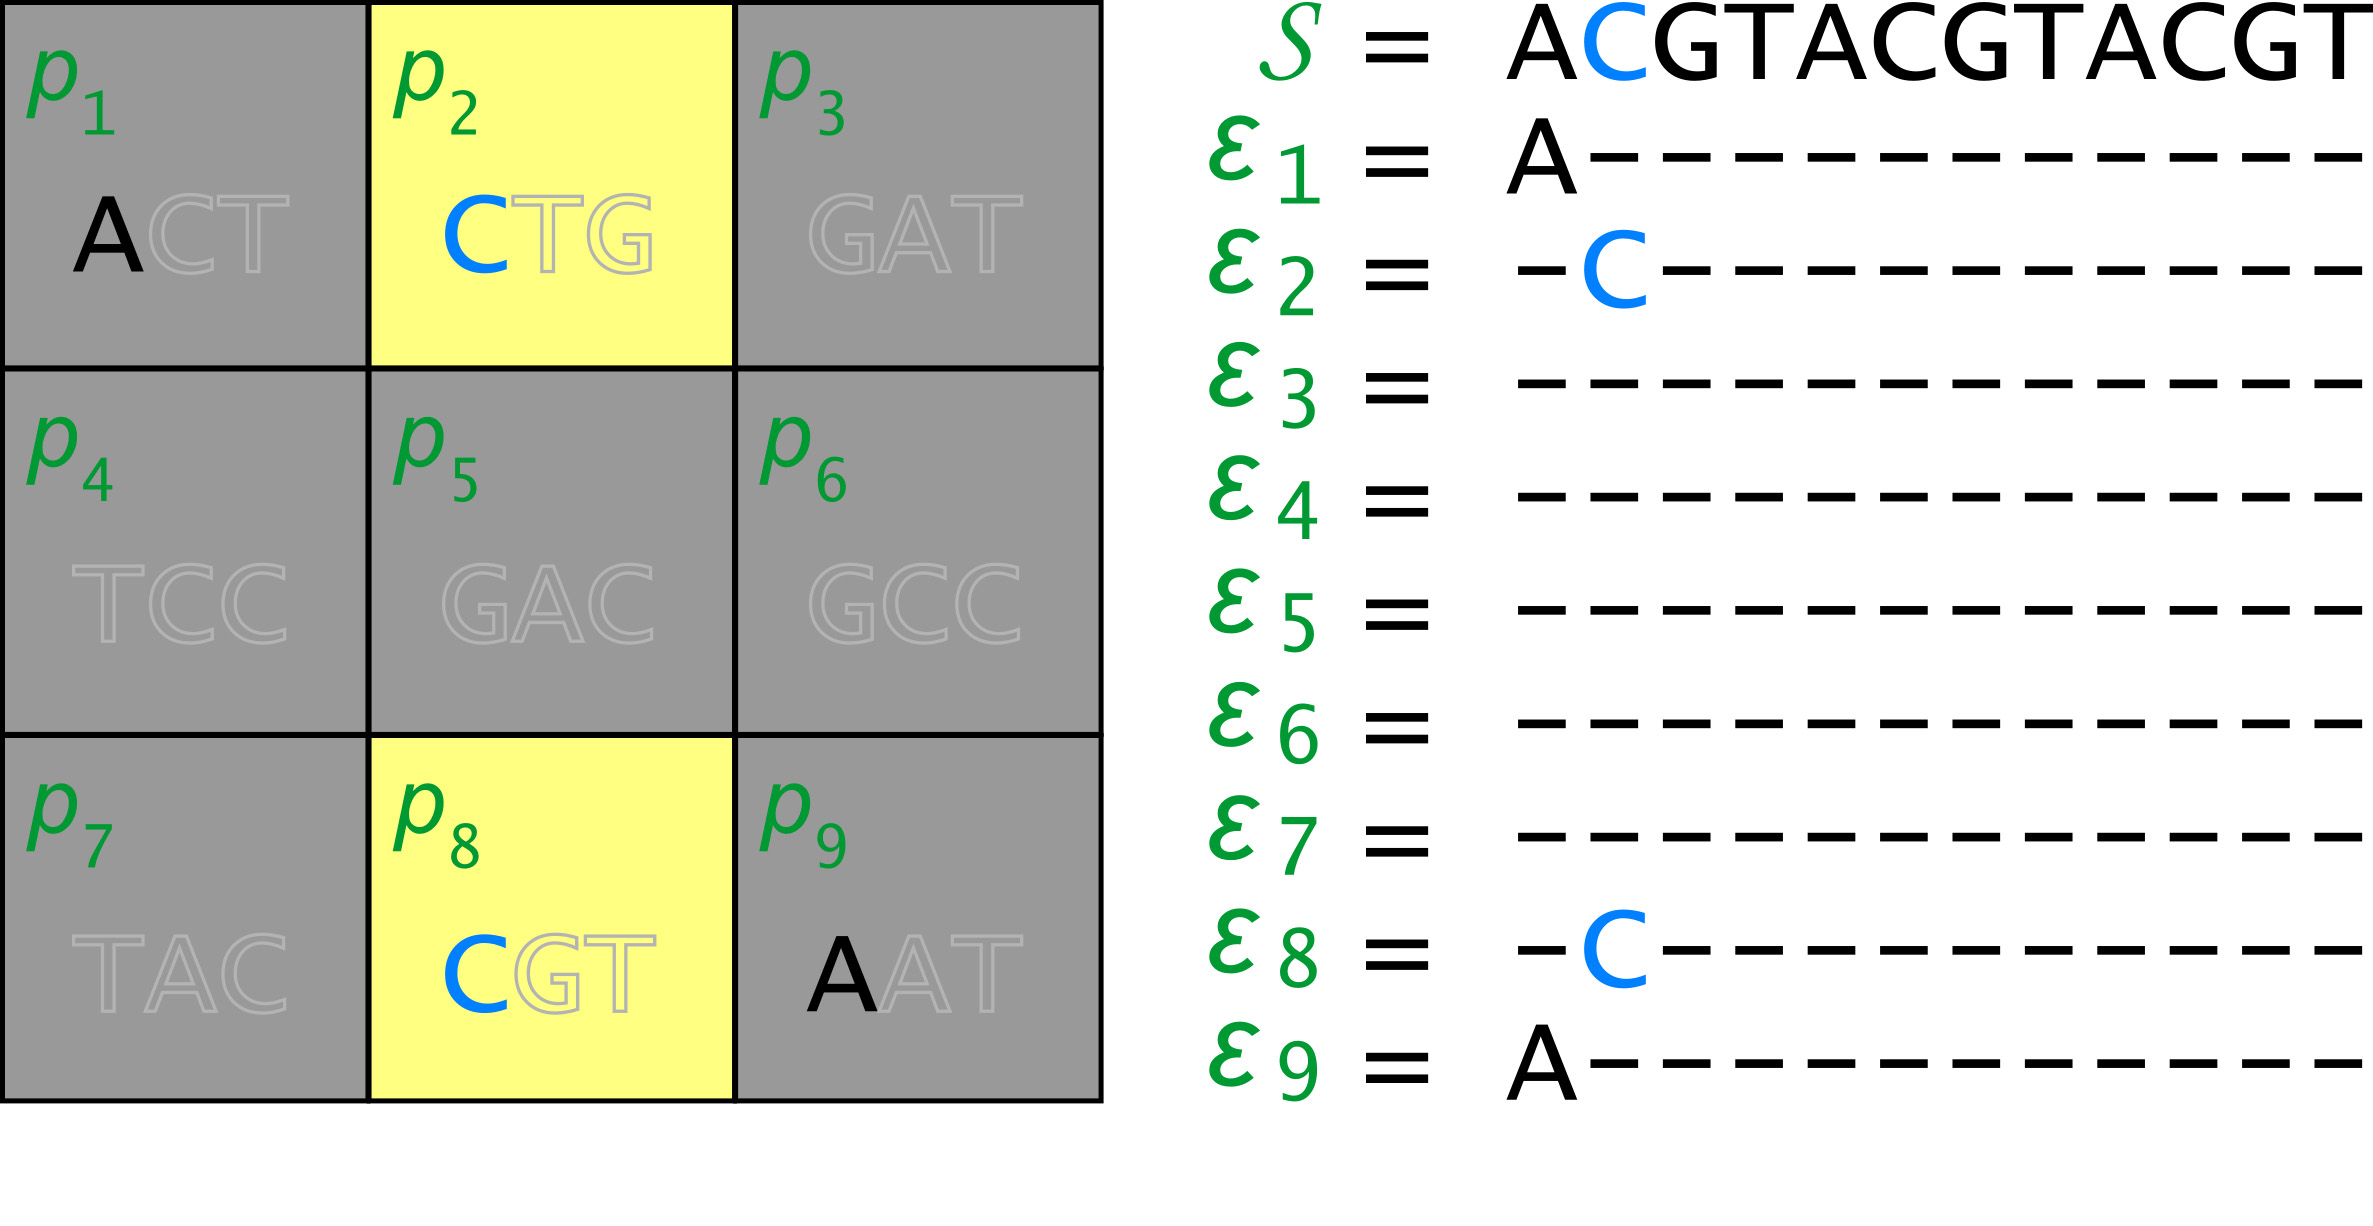
\includegraphics[width=\textwidth]{masks/mask2.jpg}
  \onslide<+>
    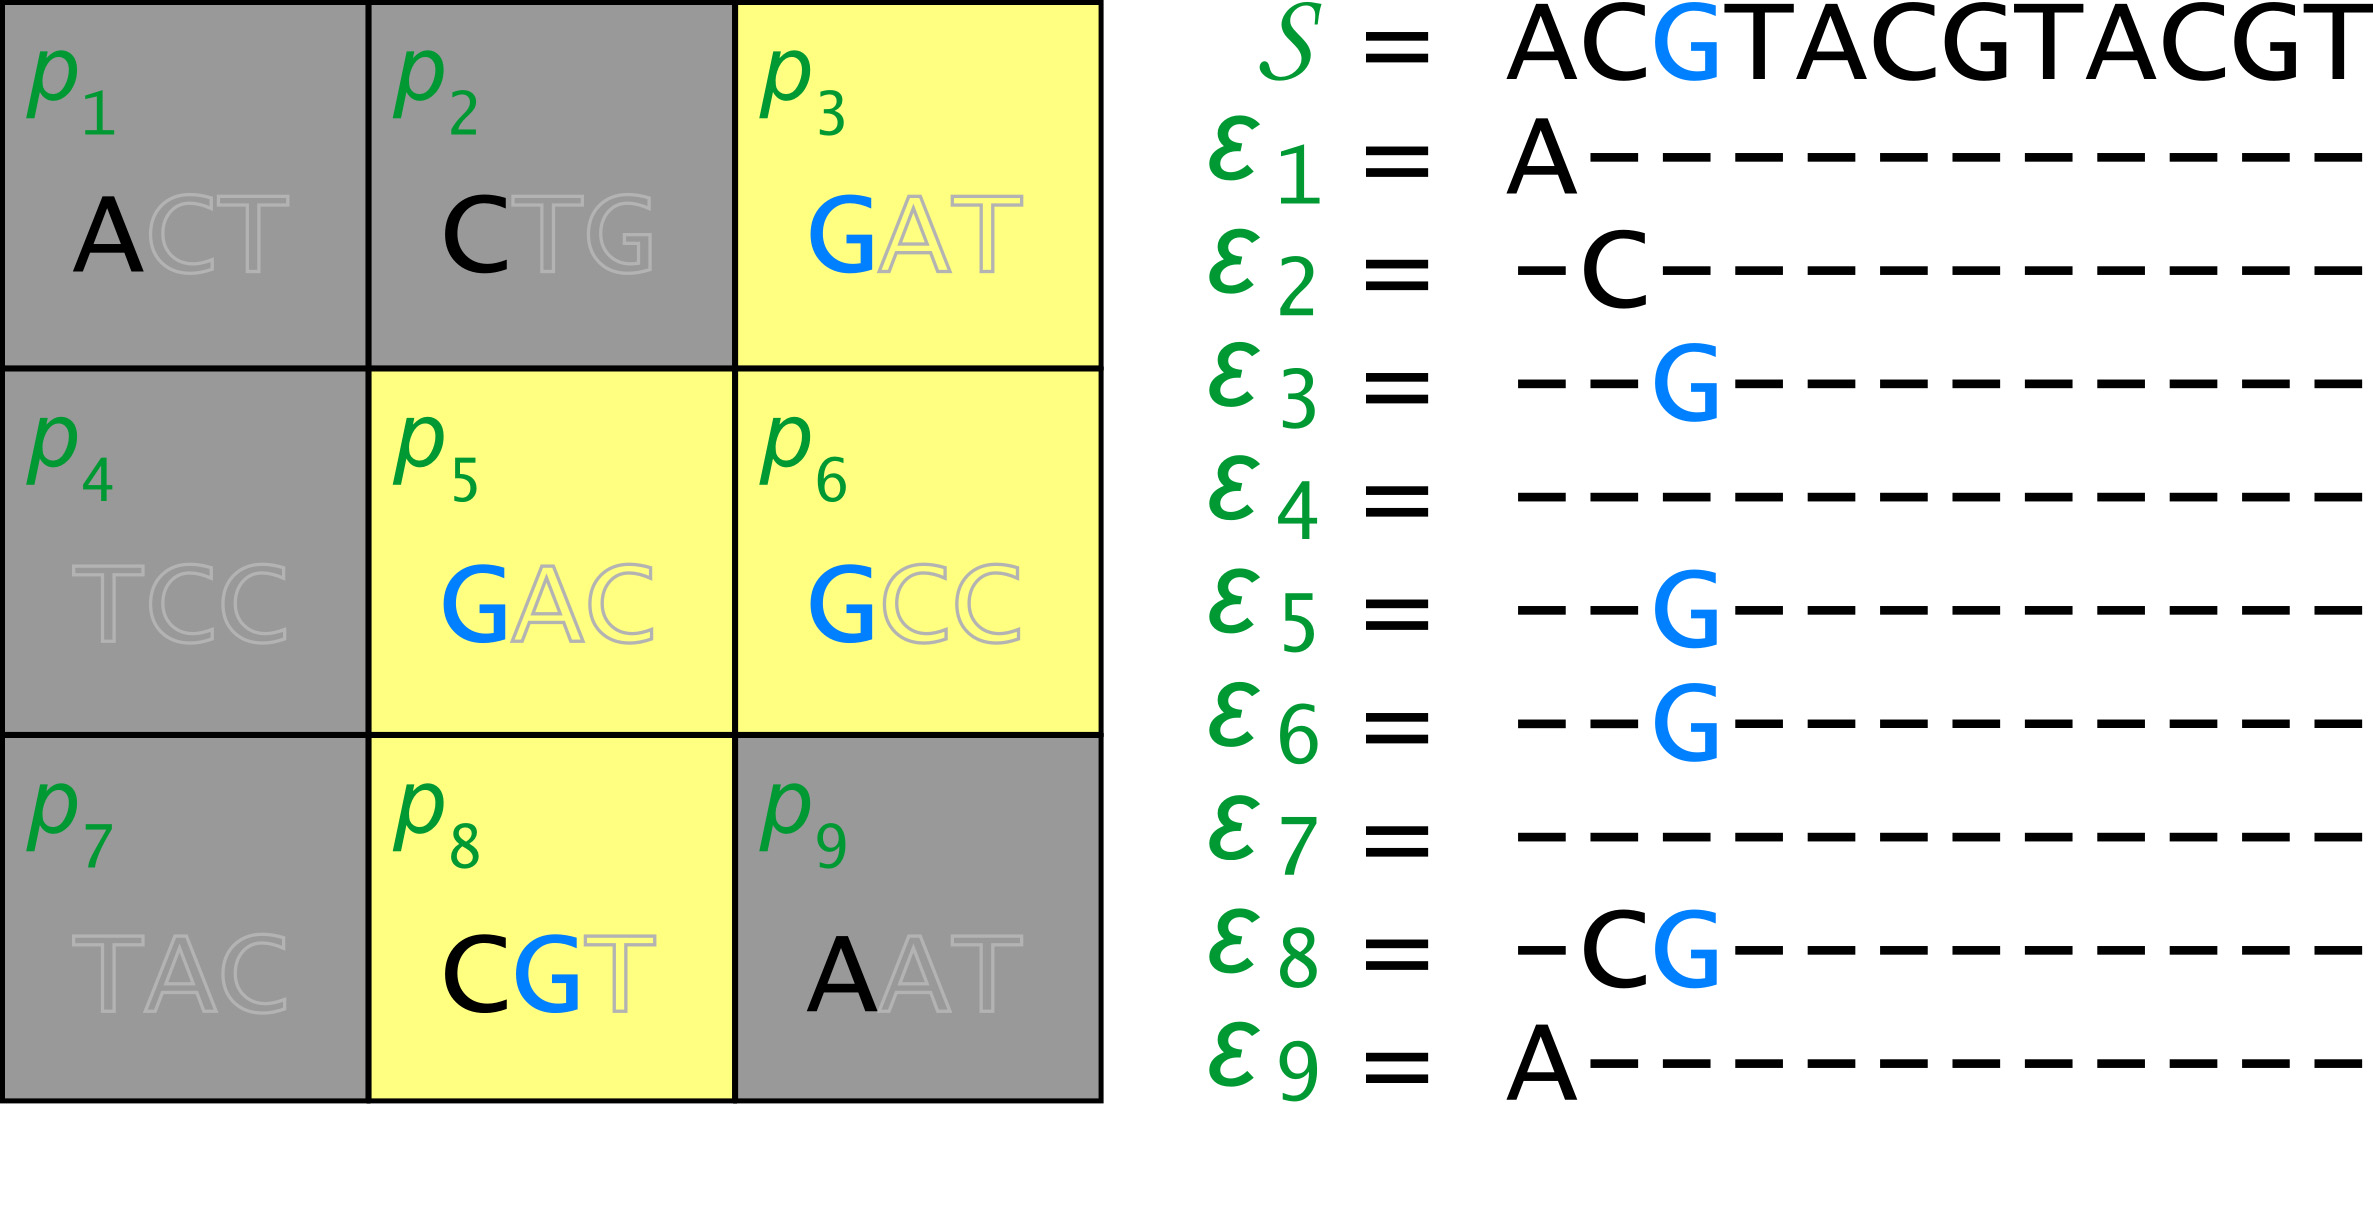
\includegraphics[width=\textwidth]{masks/mask3.jpg}
  \onslide<+>
    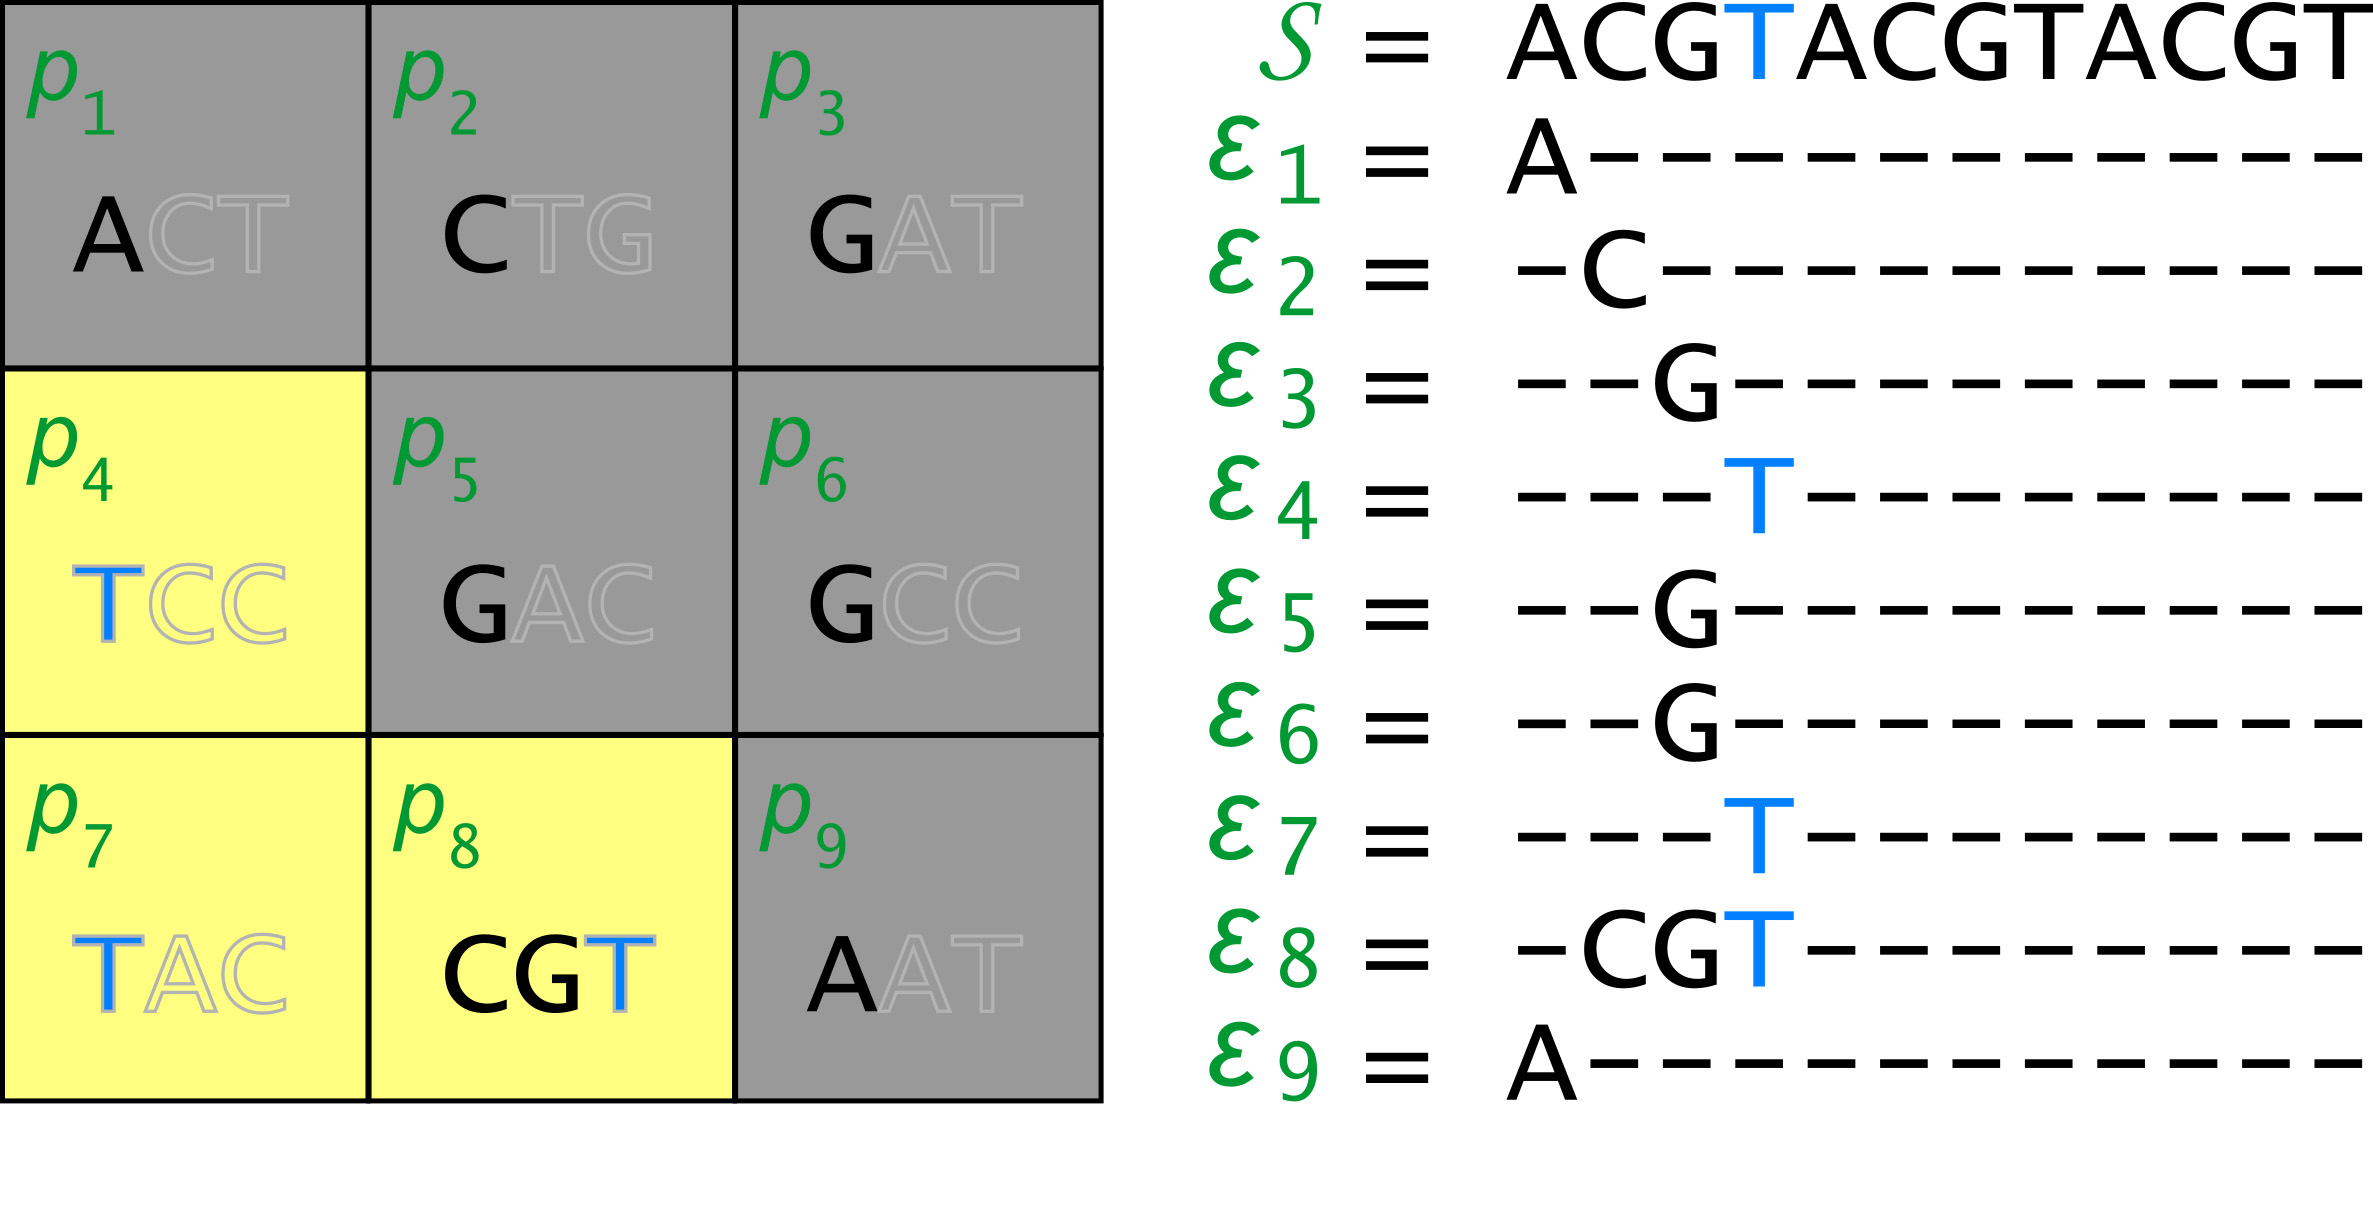
\includegraphics[width=\textwidth]{masks/mask4.jpg}
  \onslide<+>
    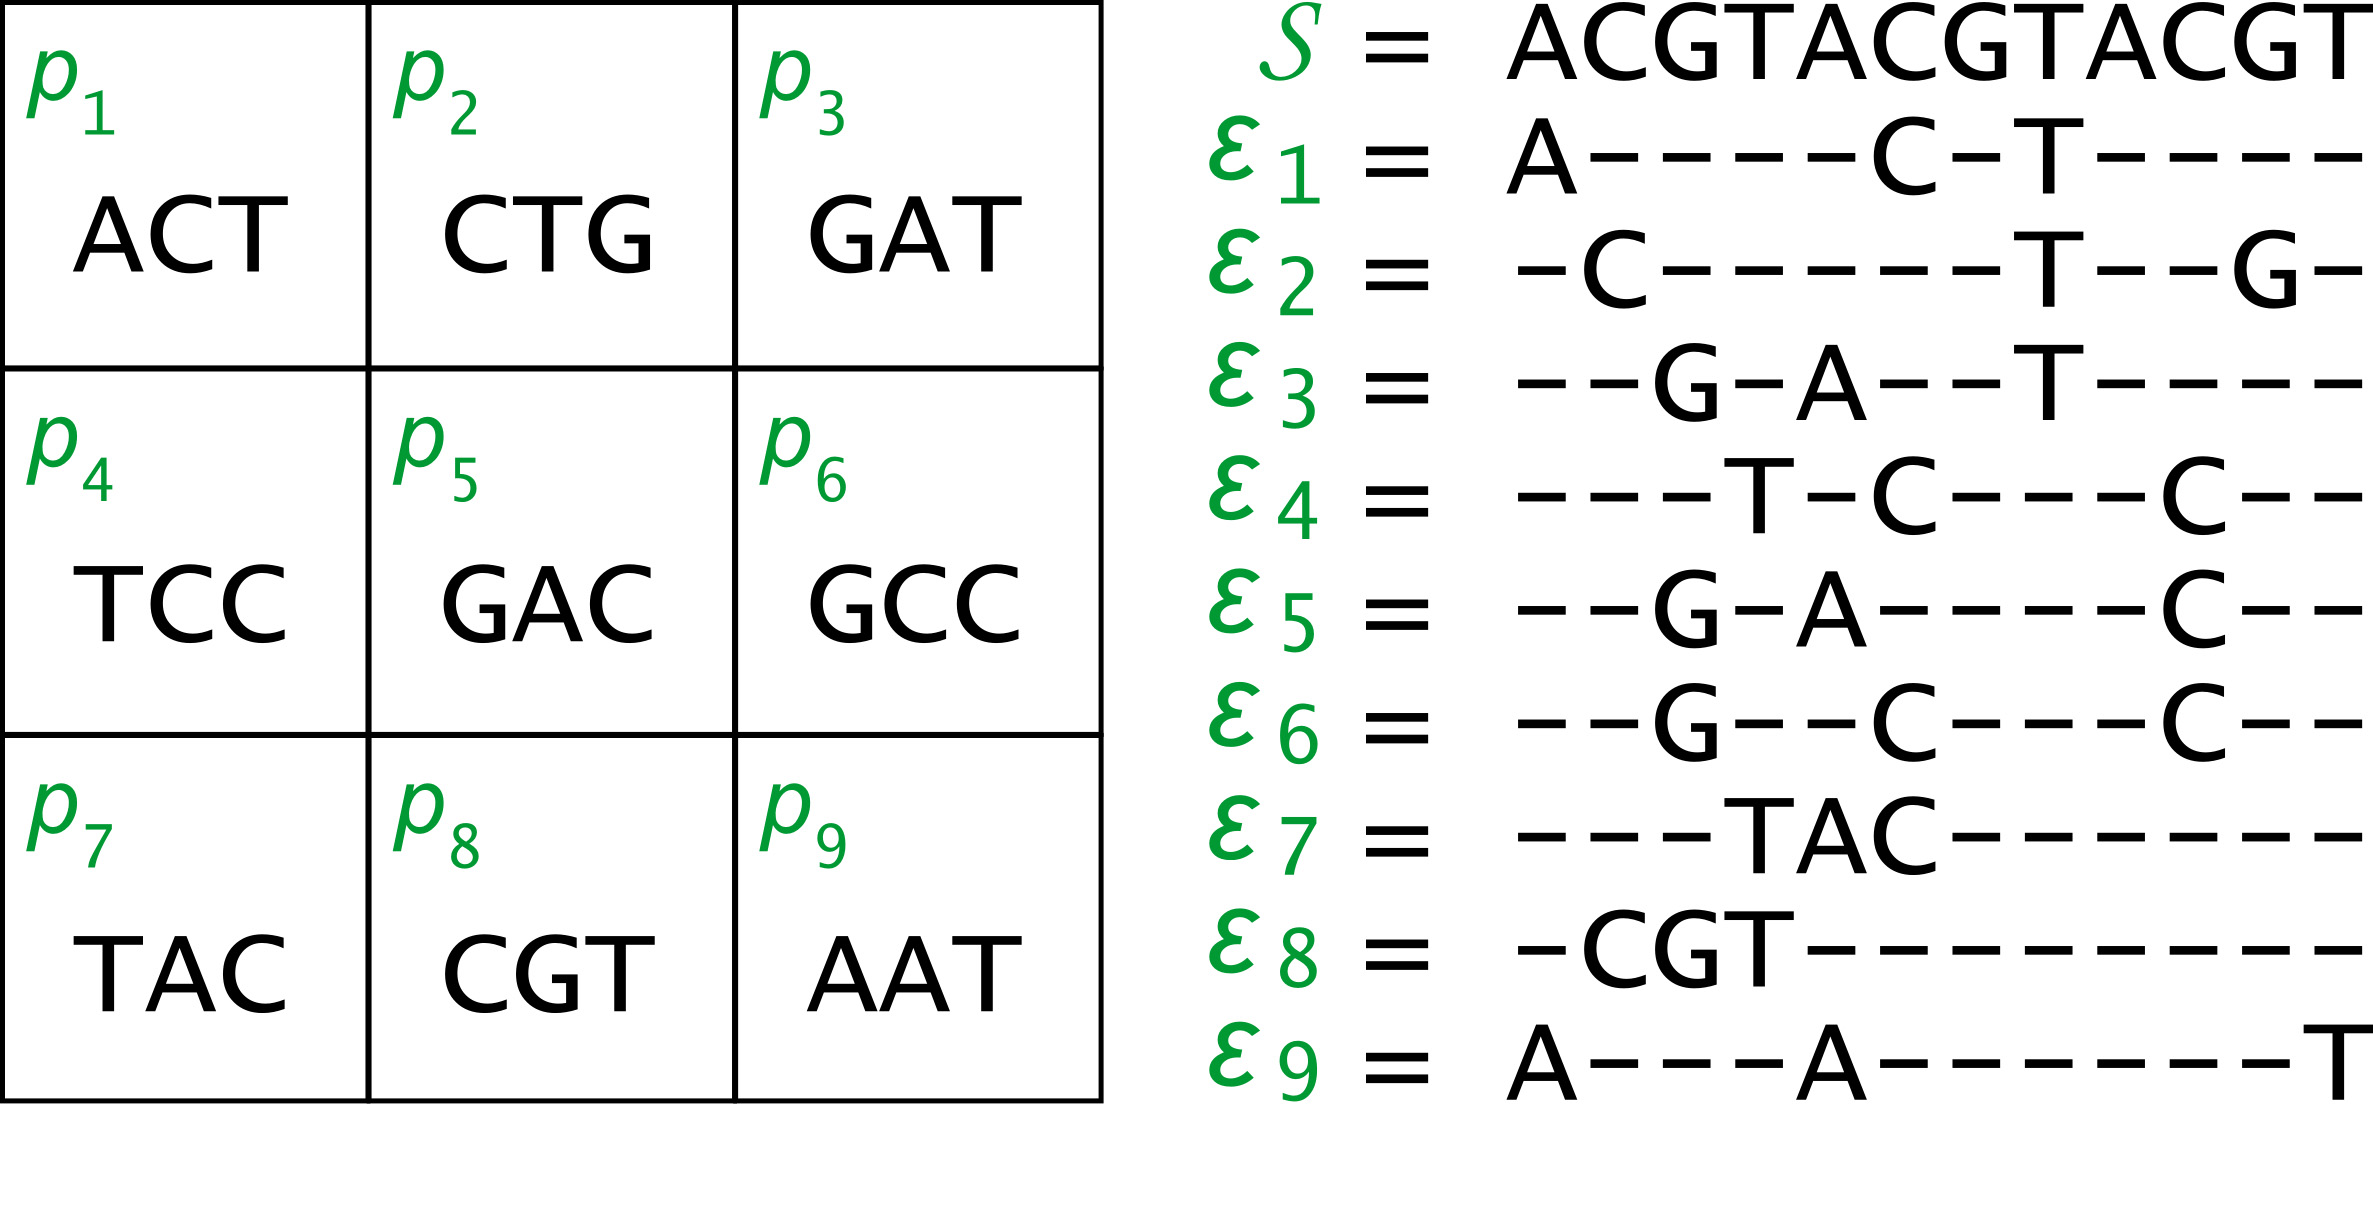
\includegraphics[width=\textwidth]{masks/embed.jpg}
  \onslide<+>
    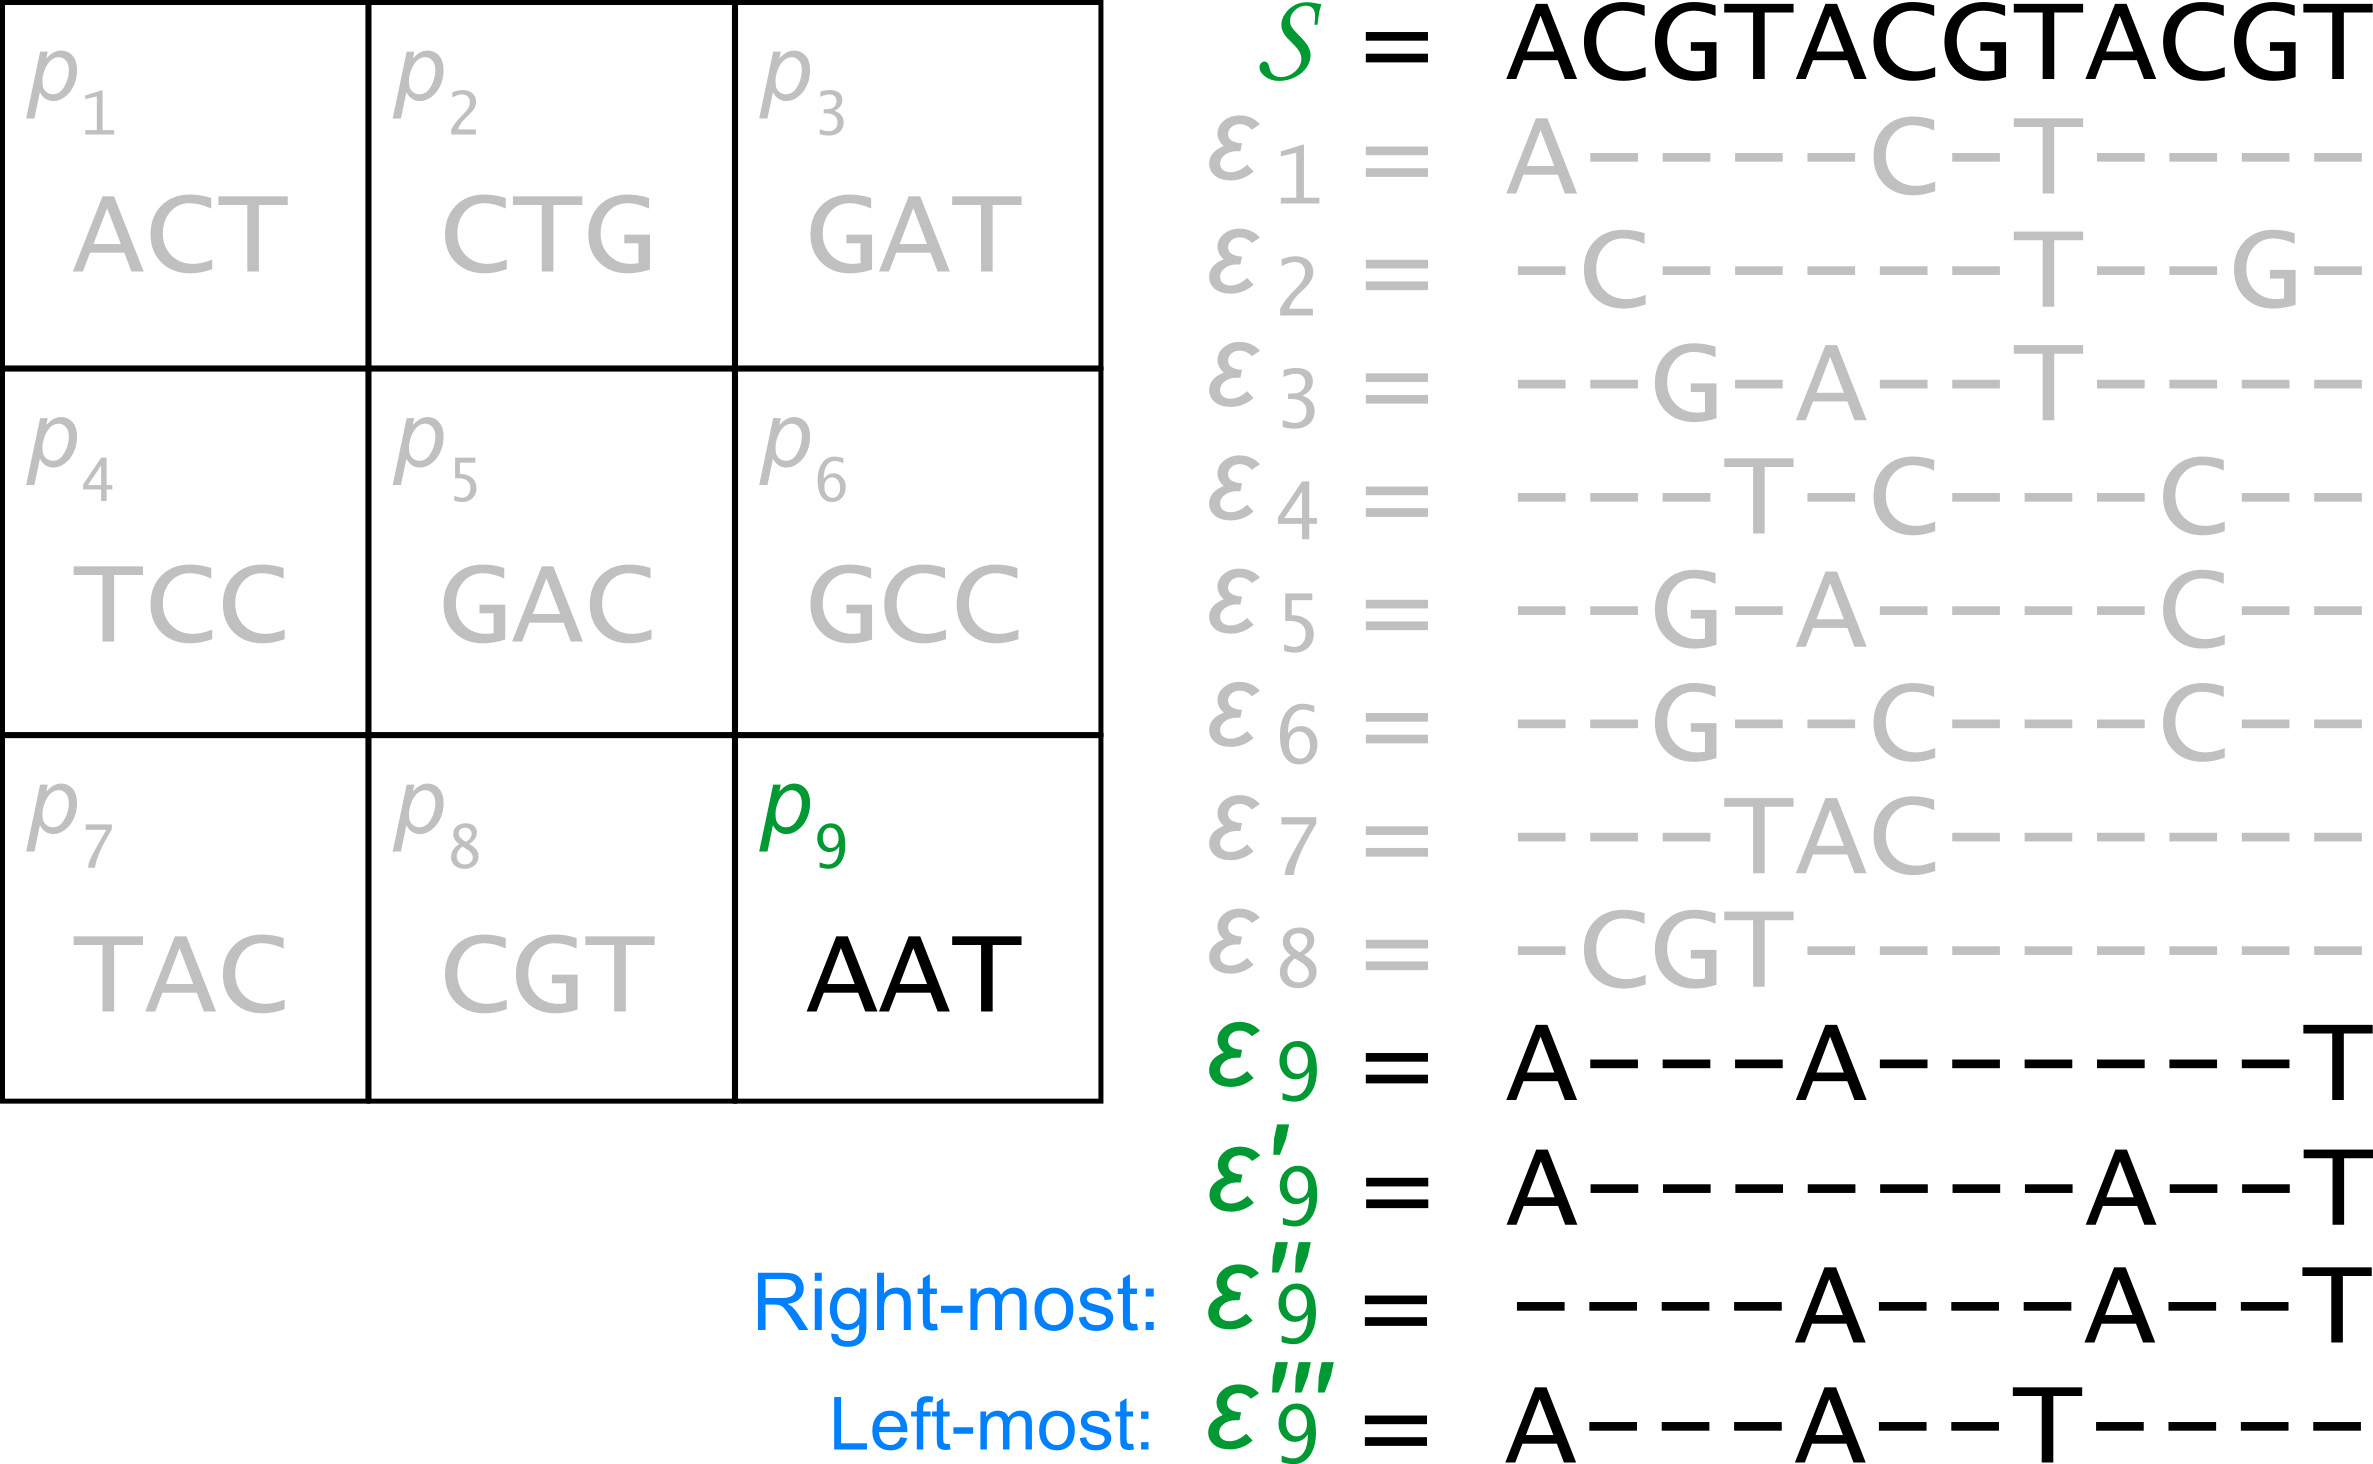
\includegraphics[width=\textwidth]{masks/alternatives.jpg}
  \end{overprint}

}

%%%%%%%%%%%%%%%%%%%%%%%%%%%%%%%%%%%%%%%%%%%%%%%%%%%%%%%%%%%%%%%%%%%%%%%%%%%%%%%%
\frame[label=problem]{\frametitle{Unintended Illumination Problem}

  \begin{columns}
  
    \begin{column}{0.45\textwidth}
      \centerline{
        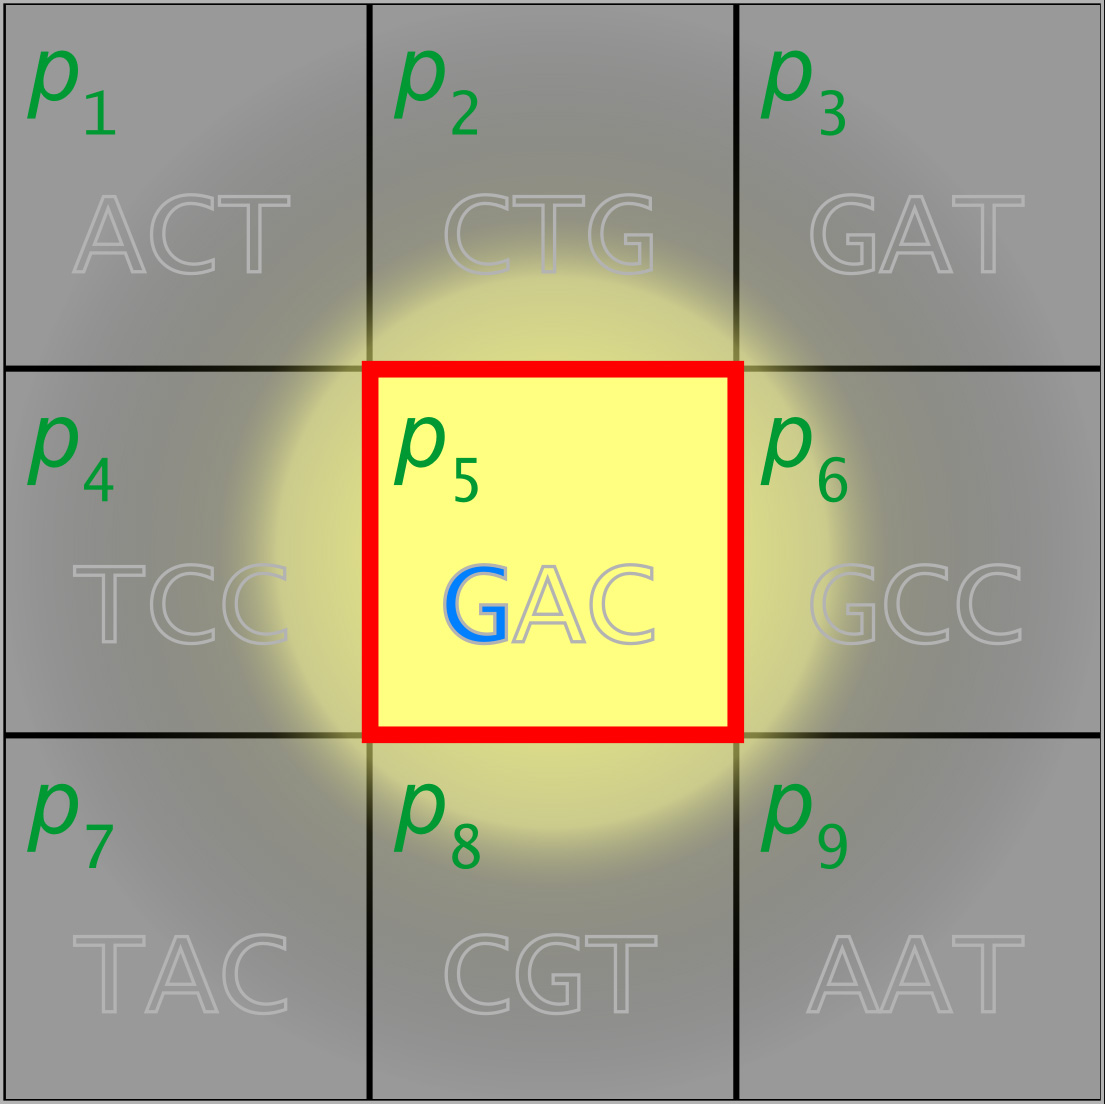
\includegraphics[width=\textwidth]{pics/straylight.jpg}
      }
    \end{column}
    
    \begin{column}{0.55\textwidth}
      \begin{itemize}
        \item \alert{Untargeted spots} can be accidentally activated
        \begin{itemize}
          \item Diffraction of light
          \item Internal reflection
        \end{itemize}
        \item Production of defective probes
        \item More likely near the \alert{borders} between masked and unmasked
              spots: \alert{border conflict}
      \end{itemize}
    \end{column}
    
  \end{columns}
  
  \begin{block}{Border Length Minimization Problem (Hannenhalli et al., 2002)}
    Find arrangement of the probes and embeddings with minimum number of border
    conflicts over all masks
  \end{block}

}

%% *****************************************************************************
\section[Conflict Index]{Conflict Index Model}
\subsection{Dummy}
%% *****************************************************************************

%%%%%%%%%%%%%%%%%%%%%%%%%%%%%%%%%%%%%%%%%%%%%%%%%%%%%%%%%%%%%%%%%%%%%%%%%%%%%%%%
\frame{\frametitle{Motivation}

  \begin{columns}  
  
    \begin{column}{0.55\textwidth}
      \begin{itemize}
        \item Border Length measures the quality of a particular mask
        \begin{itemize}
          \item We are more interested in a \alert{per-probe measure}
        \end{itemize}
        \item Practical considerations:
        \begin{itemize}
          \item[a)] Stray light might damage probes as far as \alert{three cells
                    away} from the targeted spot
          \item[b)] Imperfections \alert{in the middle} of a probe are more
                    harmful than in its extremities
        \end{itemize}
      \end{itemize}
    \end{column}
      
    \begin{column}{0.45\textwidth}
      \centerline{
        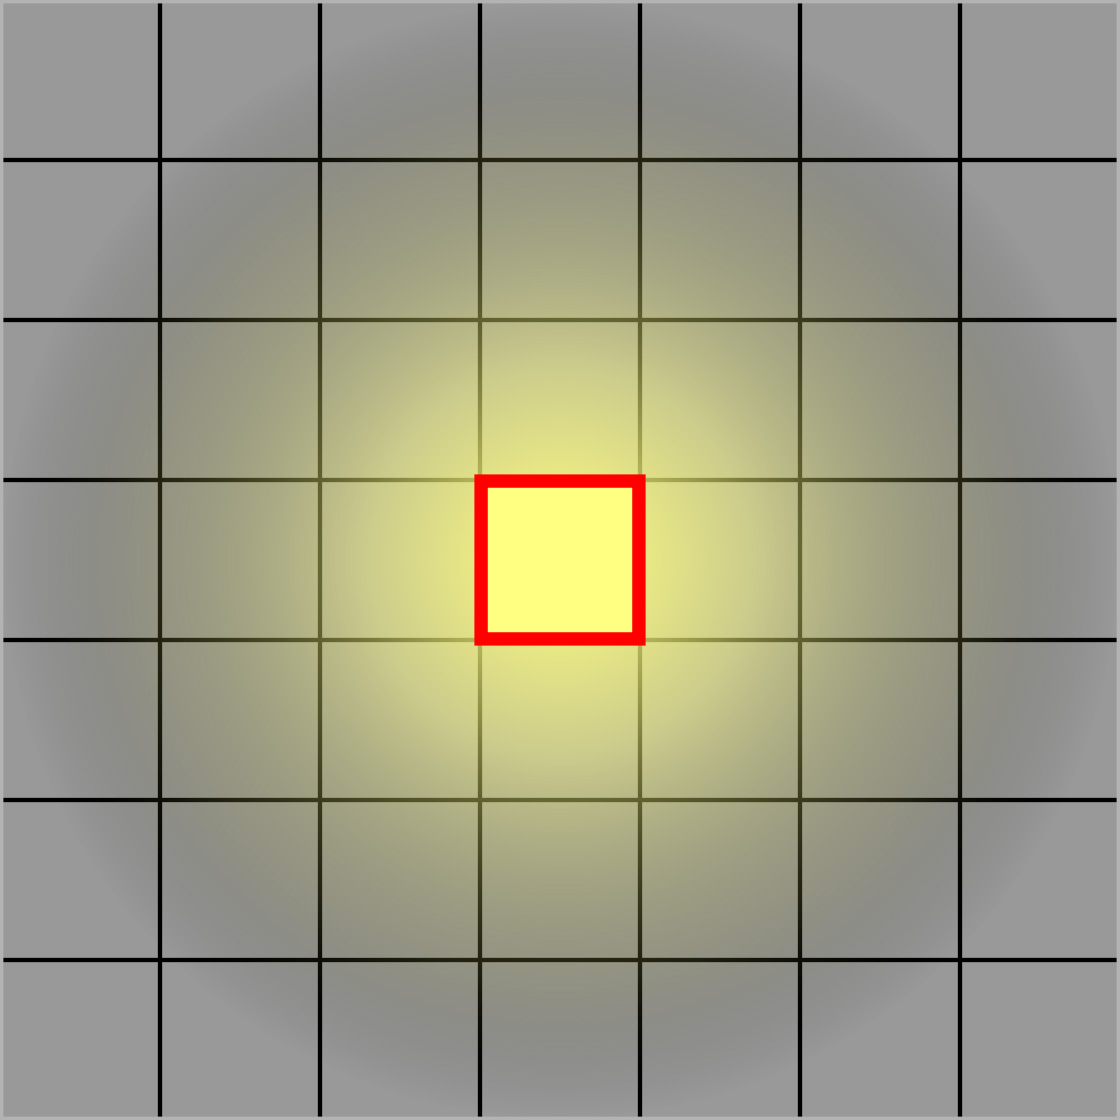
\includegraphics[width=\textwidth]{pics/distance.jpg}
      }
    \end{column}
  
  \end{columns}
  
  \vspace*{0.35cm}
  
\includegraphics[width=\textwidth]{pics/position.jpg}
}

%%%%%%%%%%%%%%%%%%%%%%%%%%%%%%%%%%%%%%%%%%%%%%%%%%%%%%%%%%%%%%%%%%%%%%%%%%%%%%%%
\frame{\frametitle{Definition}

  \begin{block}{Conflict Index of a probe $p$}
    \footnotesize{
    \[
    \mathcal{C}(p) := \sum_{t=1}^{T} \Bigl( \omega(p,t) \sum_{nbs. p'} \delta(p,p',t) \Bigr)
    \]
    }
  \end{block}
    
  \begin{block}{Distance-dependent weights}
    \footnotesize{
    \[
    \delta(p,p',t) :=
    \left\{
    \begin{array}{ll}
    (d(p,p'))^{-2} & \mbox{if $p'$ is unmasked at step $t$}, \\
                 0 & \mbox{otherwise}, \\
    \end{array}
    \right.
    \]
    %%
    where $d(p,p')$ is the \alert{Euclidean distance} between the spots of~$p$
    and~$p'$.
    }
  \end{block}

  \vspace*{0.2cm}

  \centerline{
  \scriptsize{
  \begin{tabular}{|c|c|c|c|c|c|c|c|} \hline
  0.06 & 0.08 & 0.10 & 0.11 & 0.10 & 0.08 & 0.06 \\ \hline
  0.08 & 0.13 & 0.20 & 0.25 & 0.20 & 0.13 & 0.08 \\ \hline
  0.10 & 0.20 & 0.50 & 1.00 & 0.50 & 0.20 & 0.10 \\ \hline
  0.11 & 0.25 & 1.00 & \alert{$p$} & 1.00 & 0.25 & 0.11 \\ \hline
  0.10 & 0.20 & 0.50 & 1.00 & 0.50 & 0.20 & 0.10 \\ \hline
  0.08 & 0.13 & 0.20 & 0.25 & 0.20 & 0.13 & 0.08 \\ \hline
  0.06 & 0.08 & 0.10 & 0.11 & 0.10 & 0.08 & 0.06 \\ \hline
  \end{tabular}}}
  
}

%%%%%%%%%%%%%%%%%%%%%%%%%%%%%%%%%%%%%%%%%%%%%%%%%%%%%%%%%%%%%%%%%%%%%%%%%%%%%%%%
\frame{\frametitle{Definition}

  \begin{columns}
  
    \begin{column}{0.45\textwidth}
      \begin{block}{Conflict Index of a probe $p$}
        \footnotesize{
        \[
        \mathcal{C}(p) := \sum_{t=1}^{T} \Bigl( \omega(p,t) \sum_{p'} \delta(p,p',t) \Bigr)
        \]
        }
      \end{block}
    \end{column}
    
    \begin{column}{0.45\textwidth}
      \centerline{
        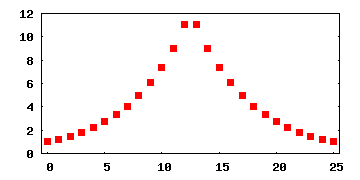
\includegraphics[width=1.25\textwidth]{pics/position_weights.png}
      }
    \end{column}
    
  \end{columns}

  \begin{block}{Position-dependent weights}
    \footnotesize{
    \[
    \omega(p,t) :=
    \left\{
    \begin{array}{ll}
    c \cdot \exp{\left(\theta \cdot \lambda(p,t)\right)} & \mbox{if $p$ is masked at step $t$}, \\
    0 & \mbox{otherwise}, \\
    \end{array}
    \right.
    \]
    %%
    where
    %%
    \[
    \lambda(p,t) := 1 + \min(b_{p,t},\ell_{p} - b_{p,t}),
    \]
    %%
    $b_{p,t}$ denotes the number of nucleotides synthesized up to and including
    step~$t$, $\ell_{p}$ is the length of probe~$p$, $c>0$ and $\theta>0$ are
    constants.
    }
  \end{block}

}

%%%%%%%%%%%%%%%%%%%%%%%%%%%%%%%%%%%%%%%%%%%%%%%%%%%%%%%%%%%%%%%%%%%%%%%%%%%%%%%%
\frame{\frametitle{New Problem}

  \begin{block}{Conflict Index Minimization Problem}
    Find placement of the probes and embeddings such that
    \footnotesize{
    \[
    \sum_{p} \mathcal{C}(p) \to \min
    \]
    }
  \end{block}

}

%% *****************************************************************************
\section[QAP Formulation]{New Approach: Quadratic Assignment Problem (QAP)}
\subsection{Dummy}
%% *****************************************************************************

%%%%%%%%%%%%%%%%%%%%%%%%%%%%%%%%%%%%%%%%%%%%%%%%%%%%%%%%%%%%%%%%%%%%%%%%%%%%%%%%
\frame{\frametitle{Previous Work: Place and Re-embed}

  The problem has been traditionally approached in two phases:
  \begin{itemize}
    \item[1)] \alert{Placement} of probes given a fixed embedding
    \item[2)] \alert{Re-embedding} of probes once a placement is fixed
  \end{itemize}
  
  \begin{block}{Placement: Row-epitaxial (Kahng {\it et~al}., 2003)}
    \begin{itemize}
      \item Spots are filled in a pre-defined order
      \begin{itemize}
        \item Select probe from a list $Q$ such that conflicts with filled spots
              are minimized
      \end{itemize}
      \item Restrict the maximum size of $Q$ (e.g. $Q = 20\,000$)
    \end{itemize}
  \end{block}

  \begin{block}{Re-embedding: Sequential (Kahng {\it et~al}., 2003)}
    \begin{itemize}
      \item Based on the Optimum Single Probe Embedding (OSPE)
      \begin{itemize}
        \item Re-embed a probe \alert{optimally} in regards to its neighbors
      \end{itemize}
      \item Spots are re-embedded in a pre-defined order
    \end{itemize}
  \end{block}
  
}

%%%%%%%%%%%%%%%%%%%%%%%%%%%%%%%%%%%%%%%%%%%%%%%%%%%%%%%%%%%%%%%%%%%%%%%%%%%%%%%%
\frame{\frametitle{Partitioning}

  \begin{itemize}
    \item The placement problem can be \alert{partitioned}
    \begin{itemize}
      \item Divide the chip into sub-regions; assign sub-sets of probes to each
            sub-region
      \item Sub-regions are processed independently, and can be
            \alert{recursively partitioned}
      \item A placement algorithm is called on each final sub-region
    \end{itemize}
    \item Partitioning is a compromise but can reduce run-time and help the
          placement algorithm
  \end{itemize}

}

%%%%%%%%%%%%%%%%%%%%%%%%%%%%%%%%%%%%%%%%%%%%%%%%%%%%%%%%%%%%%%%%%%%%%%%%%%%%%%%%
\frame{\frametitle{Partitioning}

  \begin{block}{Partitioning: Centroid Quadrisection (Kahng {\it et~al}., 2003)}
    \begin{itemize}
      \item Heuristically select four probes maximizing the Hamming distance
            between their embeddings: \alert{centroids}
      \item Chip is divided into \alert{four quadrants}, each gets one centroid
      \item Remaining probes $p$ are assigned to the quadrant whose centroid has
            the minimum Hamming distance to $p$
    \end{itemize}
  \end{block}
  
}

%%%%%%%%%%%%%%%%%%%%%%%%%%%%%%%%%%%%%%%%%%%%%%%%%%%%%%%%%%%%%%%%%%%%%%%%%%%%%%%%
\frame{\frametitle{What's New?}

  \begin{block}{Observation 1}
     \begin{itemize}
      \item Some probes have only a few possible embeddings
      \begin{itemize}
        \item Their embeddings cover most cycles of the deposition sequence
      \end{itemize}
      \item Others may have up to several million embeddings
      \begin{itemize}
        \item Particular embeddings may not serve as good centroids
      \end{itemize}
    \end{itemize}
  \end{block}
  
  \begin{block}{Pivot Partitioning}
    \begin{itemize}
      \item Restrict the selection of centroids to probes with fewer embeddings:
            \alert{pivots}
      \begin{itemize}
        \item Faster and better selection of centroids
        \item Probes with more embeddings can more ``easily'' adapt to the
              pivots
      \end{itemize}
    \end{itemize}
  \end{block}

}

%%%%%%%%%%%%%%%%%%%%%%%%%%%%%%%%%%%%%%%%%%%%%%%%%%%%%%%%%%%%%%%%%%%%%%%%%%%%%%%%
\frame{\frametitle{What's New?}

  \begin{block}{Observation 2}
    \begin{itemize}
      \item The place and re-embed approach is inefficient
      \begin{itemize}
        \item Placement is based on embeddings that are likely to change
      \end{itemize}
    \end{itemize}
  \end{block}

  \begin{block}{Pivot Partitioning}
    \begin{itemize}
      \item Consider \alert{all embeddings} when assigning probes to sub-regions
            (using OSPE)
      \begin{itemize}
        \item Better assignment of probes
      \end{itemize}
      \item \alert{Re-embed probes} in regards to the pivots \alert{before
            placement} (OSPE again)
      \begin{itemize}
        \item Improve the ``alignment'' of the embeddings in the region
      \end{itemize}      
    \end{itemize}
  \end{block}

}

%%%%%%%%%%%%%%%%%%%%%%%%%%%%%%%%%%%%%%%%%%%%%%%%%%%%%%%%%%%%%%%%%%%%%%%%%%%%%%%%
\frame{\frametitle{What's New?}

  \begin{block}{Observation 3}
    \begin{itemize}
      \item The quadrisection partitioning may force bad assignments in order to
            ensure squared regions
    \end{itemize}
  \end{block}

  \begin{block}{Pivot Partitioning}
    \begin{itemize}
      \item Alternate \alert{horizontal} and \alert{vertical} partitions
      \item Allow sub-regions to have different sizes
      \begin{itemize}
        \item Greater flexibility when assingning probes to sub-regions
      \end{itemize}
    \end{itemize}
  \end{block}

  \vspace*{0.5cm}
  
  \centerline{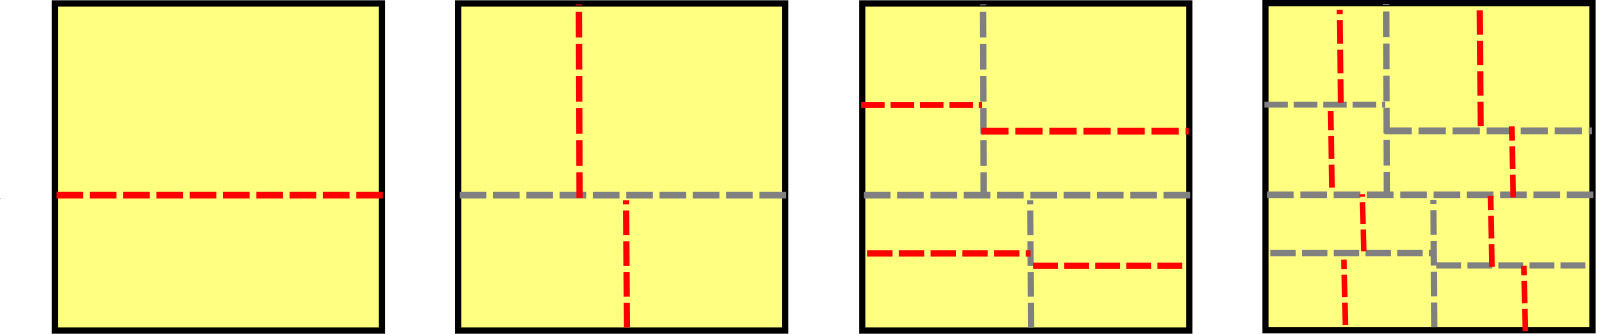
\includegraphics[width=\textwidth]{pics/pivotpart.jpg}}

}

%%%%%%%%%%%%%%%%%%%%%%%%%%%%%%%%%%%%%%%%%%%%%%%%%%%%%%%%%%%%%%%%%%%%%%%%%%%%%%%%
\frame{\frametitle{Results on Random Chips}

  Using Row-epitaxial for the placement (with $Q = 20\,000$), followed by
  Sequential re-embedding

  \begin{block}{Border Length Minimization}
    \scriptsize{
    \centerline{
    \begin{tabular}{c|rr|rr|rr|rr}
& \multicolumn{2}{c|}{$t_{max}=0$} & \multicolumn{2}{c|}{$t_{max}=2$} & \multicolumn{2}{c|}{$t_{max}=4$} & \multicolumn{2}{c}{$t_{max}=6$} \\
Dim & \multicolumn{1}{c}{Cost} & \multicolumn{1}{c|}{Time} & \multicolumn{1}{c}{Cost} & \multicolumn{1}{c|}{Time} & \multicolumn{1}{c}{Cost} & \multicolumn{1}{c|}{Time} & \multicolumn{1}{c}{Cost} & \multicolumn{1}{c}{Time} \\ \noalign{\smallskip} \hline \noalign{\smallskip}
100$\times$100 & 42.77 &     34 & 39.19 &     13 & 40.72 &     10 & 42.11 &  11 \\
200$\times$200 & 41.63 &    429 & 37.30 &    155 & 38.53 &     62 & 40.00 &  85 \\
300$\times$300 & 41.38 & 1\,174 & 36.12 &    766 & 37.22 &    264 & 38.53 & 139 \\
500$\times$500 & 41.27 & 3\,524 & 34.69 & 3\,472 & 35.50 & 1\,996 & 36.58 & 713 \\
    \end{tabular}}
    }
  \end{block}
  
  \scriptsize{
    $t_{max}$: maximum partitioning depth \\
    Dim: chip dimension \\
    Cost: \alert{normalized border length} \\
    Time: running time in seconds
  }
  
}

%%%%%%%%%%%%%%%%%%%%%%%%%%%%%%%%%%%%%%%%%%%%%%%%%%%%%%%%%%%%%%%%%%%%%%%%%%%%%%%%
\frame{\frametitle{Results on Random Chips}

  Using Row-epitaxial for the placement (with $Q = 2\,000$), followed by
  Sequential re-embedding

  \begin{block}{Conflict Index minimization}
    \scriptsize{
    \centerline{
    \begin{tabular}{c|rr|rr|rr|rr}
& \multicolumn{2}{c|}{$t_{max}=0$} & \multicolumn{2}{c|}{$t_{max}=2$} & \multicolumn{2}{c|}{$t_{max}=4$} & \multicolumn{2}{c}{$t_{max}=6$} \\
Dim & \multicolumn{1}{c}{Cost} & \multicolumn{1}{c|}{Time} & \multicolumn{1}{c}{Cost} & \multicolumn{1}{c|}{Time} & \multicolumn{1}{c}{Cost} & \multicolumn{1}{c|}{Time} & \multicolumn{1}{c}{Cost} & \multicolumn{1}{c}{Time} \\ \noalign{\smallskip} \hline \noalign{\smallskip}
100$\times$100 & 514.49 &     45 & 453.67 &     37 & 467.78 &     19 & 475.44 &     15 \\
200$\times$200 & 517.07 &    192 & 466.22 &    215 & 452.41 &    166 & 462.55 &     99 \\
300$\times$300 & 518.51 &    438 & 475.84 &    524 & 452.00 &    466 & 448.17 &    336 \\
500$\times$500 & 517.50 & 1\,471 & 481.36 & 1\,530 & 462.33 & 1\,472 & 445.43 & 1\,295 \\
    \end{tabular}}
    }
  \end{block}

  \scriptsize{
    $t_{max}$: maximum partitioning depth \\
    Dim: chip dimension \\
    Cost: \alert{average conflict index} \\
    Time: running time in seconds
  }

}

%% *****************************************************************************
\section*{Summary}
\subsection*{Dummy}
%% *****************************************************************************

%%%%%%%%%%%%%%%%%%%%%%%%%%%%%%%%%%%%%%%%%%%%%%%%%%%%%%%%%%%%%%%%%%%%%%%%%%%%%%%%
\frame{\frametitle{Summary}

  \begin{itemize}
    \item \alert{Conflict Index}
    \begin{itemize}
      \item New model for evaluating microarray layouts
    \end{itemize}
    \item \alert{New approach to placement}
  \end{itemize}
  
  \vspace*{0.3cm}
  \begin{itemize}
    \item Challenges
    \begin{itemize}
      \item Use it as a post-placement optimization
      \item Formulation considering all embeddings
    \end{itemize}
  \end{itemize}

}

%%%%%%%%%%%%%%%%%%%%%%%%%%%%%%%%%%%%%%%%%%%%%%%%%%%%%%%%%%%%%%%%%%%%%%%%%%%%%%%%
\frame{\frametitle{Auf Wiedersehen!}

  \begin{block}{More info on}
    \centerline{\tt\alert{
      http://gi.cebitec.uni-bielefeld.de/assb/chiplayout
    }}
  \end{block}

  \begin{block}{QAPLIB}
    \centerline{\tt\alert{
      http://www.seas.upenn.edu/qaplib
    }}
  \end{block}

  \begin{itemize}
    \item Thanks to Peter Hahn (University of Pennsylvania, USA)
    \item And \alert{thank you} for your attention!
  \end{itemize}
  
}

\end{document}
